% Ref: https://www.overleaf.com/latex/templates/emory-poster-template/skpfmpxjnqdh

\documentclass[25pt, a0paper, landscape, margin=10mm, innermargin=15mm, blockverticalspace=10mm, subcolspace=7mm, dvipsnames]{tikzposter} % you need to leave in dvipsnames or else it undoes the orange edge colour??

\usepackage[T1]{fontenc}
\usepackage{helvet}
%\usepackage[utf8]{inputenc}
\usepackage{amsmath}
\usepackage{amsfonts}
\usepackage{amsthm}
\usepackage{amssymb}
\usepackage{mathrsfs}
\usepackage{graphicx}
\usepackage{adjustbox}
\usepackage{enumitem}
\usepackage[backend=bibtex,style=numeric, citestyle=ieee]{biblatex}
\usepackage{xpatch}
\usepackage{xcolor}
\usepackage{multicol}
\usepackage{lipsum}
\usepackage{setspace}
\usepackage{tcolorbox}

\setlength{\columnsep}{2.3cm}
\setlength{\columnseprule}{1mm}
\pagecolor{Dandelion}

% Ref: https://latex-cookbook.net/poster/
\renewcommand*{\familydefault}{\sfdefault}% Let's have a sans serif font

% set theme parameters
\tikzposterlatexaffectionproofoff
\usepackage{anyfontsize}
\usetheme{Default}
\usebackgroundstyle{Default}
\definecolor{epccnavy}{HTML}{1D2A3D}
\definecolor{universityred}{HTML}{D50032}
\colorlet{backgroundcolor}{white} % <<< this makes bg white
\colorlet{framecolor}{epccnavy}%Dandelion}
\colorlet{titlefgcolor}{epccnavy}
\colorlet{blocktitlebgcolor}{epccnavy}
\colorlet{blocktitlefgcolor}{white}
\colorlet{blockframecolor}{epccnavy}

% \definetitlestyle{sampletitle}{
%     width=800mm, 
%     roundedcorners=20, 
%     linewidth=10pt, 
%     innersep=10pt,
%     titletotopverticalspace=15mm, titletoblockverticalspace=25mm 
% }{
% \begin{scope}[line width=\titlelinewidth, rounded corners=\titleroundedcorners]
% \draw[color=blocktitlebgcolor, fill=titlebgcolor]
% (\titleposleft,\titleposbottom) rectangle (\titleposright,\titlepostop);
% \end{scope}
% }
% \usetitlestyle[]{sampletitle}


% Ref: https://tex.stackexchange.com/questions/309713/modify-font-style-in-title-of-tikzposter
\settitle{ \centering
\vbox{
    \begin{spacing}{1.2}
    %\@titlegraphic \\[\TP@titlegraphictotitledistance] \centering
    \color{titlefgcolor} {\sffamily \bfseries \huge  \textsc{\@title} \par}
    \vspace*{0.75em}
    \color{universityred} {\sffamily \bfseries \huge \subtitle}   
    %\vspace*{0.2em}
    \begin{flushleft}
    {\color{titlefgcolor} {\sffamily \huge \@author}
    \hspace{0.4em}
    {\sffamily \LARGE \@institute \par}}
    \end{flushleft}
    \end{spacing}
}
}
\makeatother

% Ref: https://tex.stackexchange.com/questions/180234/how-can-i-make-my-title-wrap-in-a-tikzposter
\makeatletter
\def\title#1{\gdef\@title{\scalebox{\TP@titletextscale}{%
			\begin{minipage}[t]{\linewidth}
				%\centering
				#1
			\par
				\vspace{0.5em}
			\end{minipage}%
}}}
\makeatother

% Ref: https://tex.stackexchange.com/questions/263563/add-logos-beyond-the-title-tikzposter
\title{\parbox{\linewidth}{\fontseries{bx}\selectfont {\fontsize{85}{85}\selectfont {Identifying Developer Personas Could Create \\ Better Research Software Development} }}}
\newcommand{\subtitle}{Are YOU an RS-10X? Mining GitHub to Describe Developer/Repository Interaction Types}
\author{\textbf{Felicity `Flic' Anderson\textsuperscript{$\dagger$}, Dr. Julien Sindt\textsuperscript{$\dagger$} \& Prof. Neil Chue Hong\textsuperscript{$\dagger$}}}
\institute{\textsuperscript{$\dagger$}EPCC, University of Edinburgh}
%\titlegraphic{
\includegraphics{epcclogo.png}}

\makeatletter
\newcommand\insertlogoi[2][]{\def\@insertlogoi{\includegraphics[#1]{#2}}}
%\newcommand\insertlogoi[2][]{\def\@insertlogoi{\hspace*{0.5in}\includegraphics[#1]{#2}}}
\newcommand\insertlogoii[2][]{\def\@insertlogoii{\includegraphics[#1]{#2}}}
%\newcommand\insertlogoii[2][]{\def\@insertlogoii{\hspace*{-7.5in}\includegraphics[#1]{#2}}}
%\newcommand\insertlogoiii[2][]{\def\@insertlogoiii{\includegraphics[#1]{#2}}}
\newlength\LogoSep
\setlength\LogoSep{0pt}

\insertlogoi[width=14cm]{informaticsUoE.png}
\insertlogoii[width=15cm]{epcclogo.png}
%\insertlogoii[width=15cm]{EpccANDEmailQRsidebyside.png}

\renewcommand\maketitle[1][width=800mm, linewidth=6pt]{  % #1 keys
	\normalsize
	\setkeys{title}{#1}
	% Title dummy to get title height
	\node[transparent,inner sep=\TP@titleinnersep, line width=\TP@titlelinewidth, anchor=north, minimum width=\TP@visibletextwidth-2\TP@titleinnersep]
	(TP@title) at ($(0, 0.5\textheight-\TP@titletotopverticalspace)$) {\parbox{\TP@titlewidth-2\TP@titleinnersep}{\TP@maketitle}};
	\draw let \p1 = ($(TP@title.north)-(TP@title.south)$) in node {
		\setlength{\TP@titleheight}{\y1}
		\setlength{\titleheight}{\y1}
		\global\TP@titleheight=\TP@titleheight
		\global\titleheight=\titleheight
	};
	
	% Compute title position
	\setlength{\titleposleft}{-0.5\titlewidth}
	\setlength{\titleposright}{\titleposleft+\titlewidth}
	\setlength{\titlepostop}{0.5\textheight-\TP@titletotopverticalspace}
	\setlength{\titleposbottom}{\titlepostop-\titleheight}
	
	% Title style (background)
	\TP@titlestyle
	
	% Title node
	\node[inner sep=\TP@titleinnersep, line width=\TP@titlelinewidth, anchor=north, minimum width=\TP@visibletextwidth-2\TP@titleinnersep]
	at (0,0.5\textheight-\TP@titletotopverticalspace)
	(title)
	{\parbox{\TP@titlewidth-2\TP@titleinnersep}{\TP@maketitle}};
	
	\node[inner sep=0pt,anchor=west] 
	at ([xshift=-\LogoSep]title.west)
	{\@insertlogoi};
	
	\node[inner sep=0pt,anchor=east] 
	at ([xshift=\LogoSep]title.east)
	{\@insertlogoii};
	
	% Settings for blocks
	\normalsize
	\setlength{\TP@blocktop}{\titleposbottom-\TP@titletoblockverticalspace}
}
\makeatother

\onehalfspacing
% begin document
\begin{document}
%\useblockstyle{Basic}
\maketitle
\begin{columns}
\column{.49}

\block[linewidth=5pt]{0: Identifying the Habits of Highly Effective Developers}{
    \vspace{0.4em}
    {\fontsize{42}{42}\selectfont 
    %\vspace{1em}
    \textbf{This pilot study attempts to identify `superstar developers' within 10 larger RS repositories by exploring assignment and contributions data.}
    \vspace{0.7em}
    \begin{itemize}
    \setlength{\itemindent}{0.5em}
    \setlength\itemsep{0.2em}
        \item Assignment to GitHub features \textbf{Issue Tickets and Pull Requests} (PRs) correlate with commit contributions.
        \item Individually limited metrics can be combined to give better picture of development responsibilities or activity.
        \item \textbf{Can this approach locate distinct clusters of behaviours and define and describe RS developer personas? Can they predict effectiveness?} 
    \end{itemize}
    %\vspace{1em}
    }
    %{\fontsize{45}{45}\selectfont
    %This pilot study attempts to identify `superstar developers' within 10 larger RS repositories by exploring assignment and contributions data.  
    %\vspace{1em}
    %}        % via https://tex.stackexchange.com/a/499070
} 
\block[linewidth=5pt]{1: Mining RS Repository Data To Understand Dev/Repo Interactions}{
    \begin{multicols}{2}
    \vspace{1em}
    {\fontsize{32}{32}\selectfont 
        \begin{tikzfigure}
            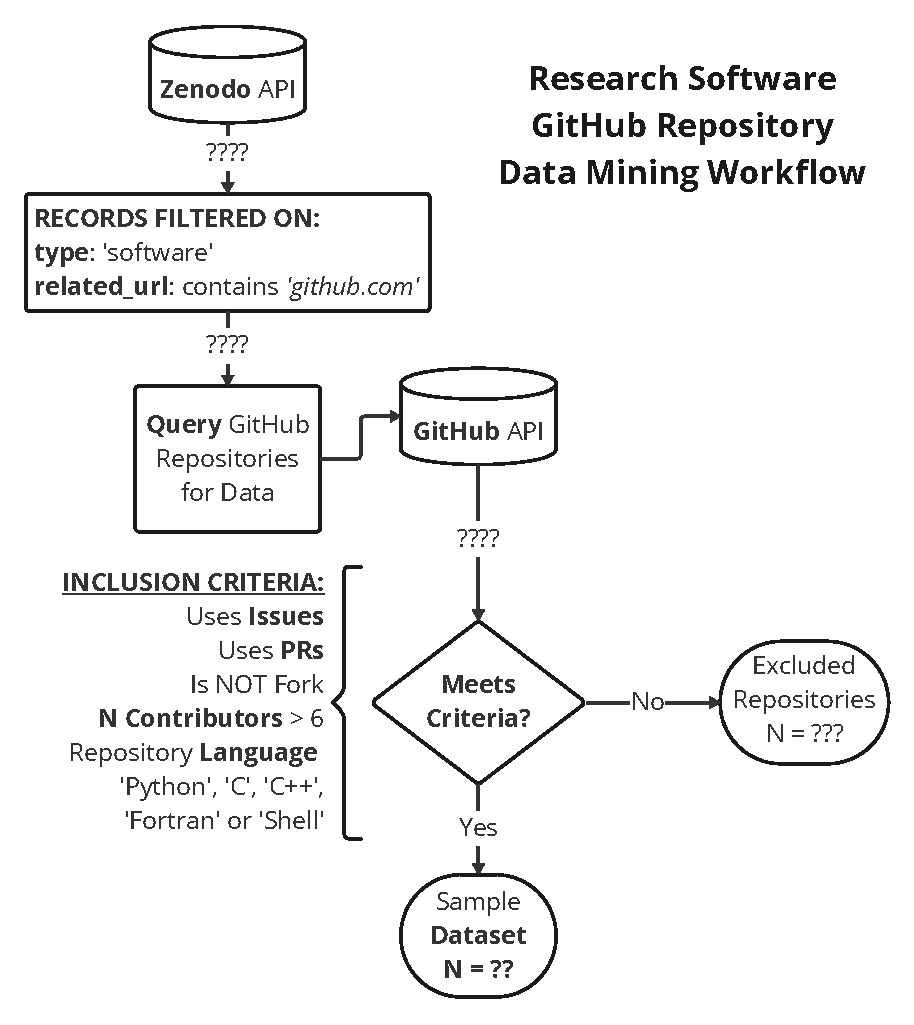
\includegraphics[height=290mm]{Figures/epccposter - DataMiningWorkflow.pdf}
        \end{tikzfigure}
        \columnbreak
        Research Software (RS) is any software used to generate research, across academic fields. 
        \vspace{1em}
        
        Public GitHub projects with a DOI (often required for publication) across all fields have been used.
        \vspace{0.4em}
        \begin{tikzfigure}[]
        %\setlength{\belowcaptionskip}{-8pt}
            \includegraphics[width=0.96\linewidth]{Figures/bars_usage.png}
        \end{tikzfigure}
        
        Of 1823 repositories identified from Zenodo, only 31\% use Issue Tickets or Pull Requests (35\%).}
    {\fontsize{32}{32}\selectfont
    \begin{tcolorbox}[colframe=white,colback=epccnavy!08, linewidth=0.8*linewidth]{   
        Assignment and Commit data were gathered from \textbf{10 larger repositories} to form a pilot study dataset. 
        \par
        Developers were grouped by \textbf{`assignment categories'}, defined as \textit{being assigned to 1+ Issue and/or 1+ PR}
    }
   \end{tcolorbox}}
    \end{multicols}
}
\block[linewidth=3pt]{}{
    \textbf{Contact: Felicity.Anderson@ed.ac.uk} \hspace{0.5em} 
    \textbf{Acknowledgements:} Work funded by a EPSRC DTA Scholarship.
    }

\column{.51}
\block[linewidth=5pt]{2: More Responsibility = More Action?}{
    \begin{multicols}{2}
    \begin{tikzfigure}[]
        %\setlength{\belowcaptionskip}{-8pt}
            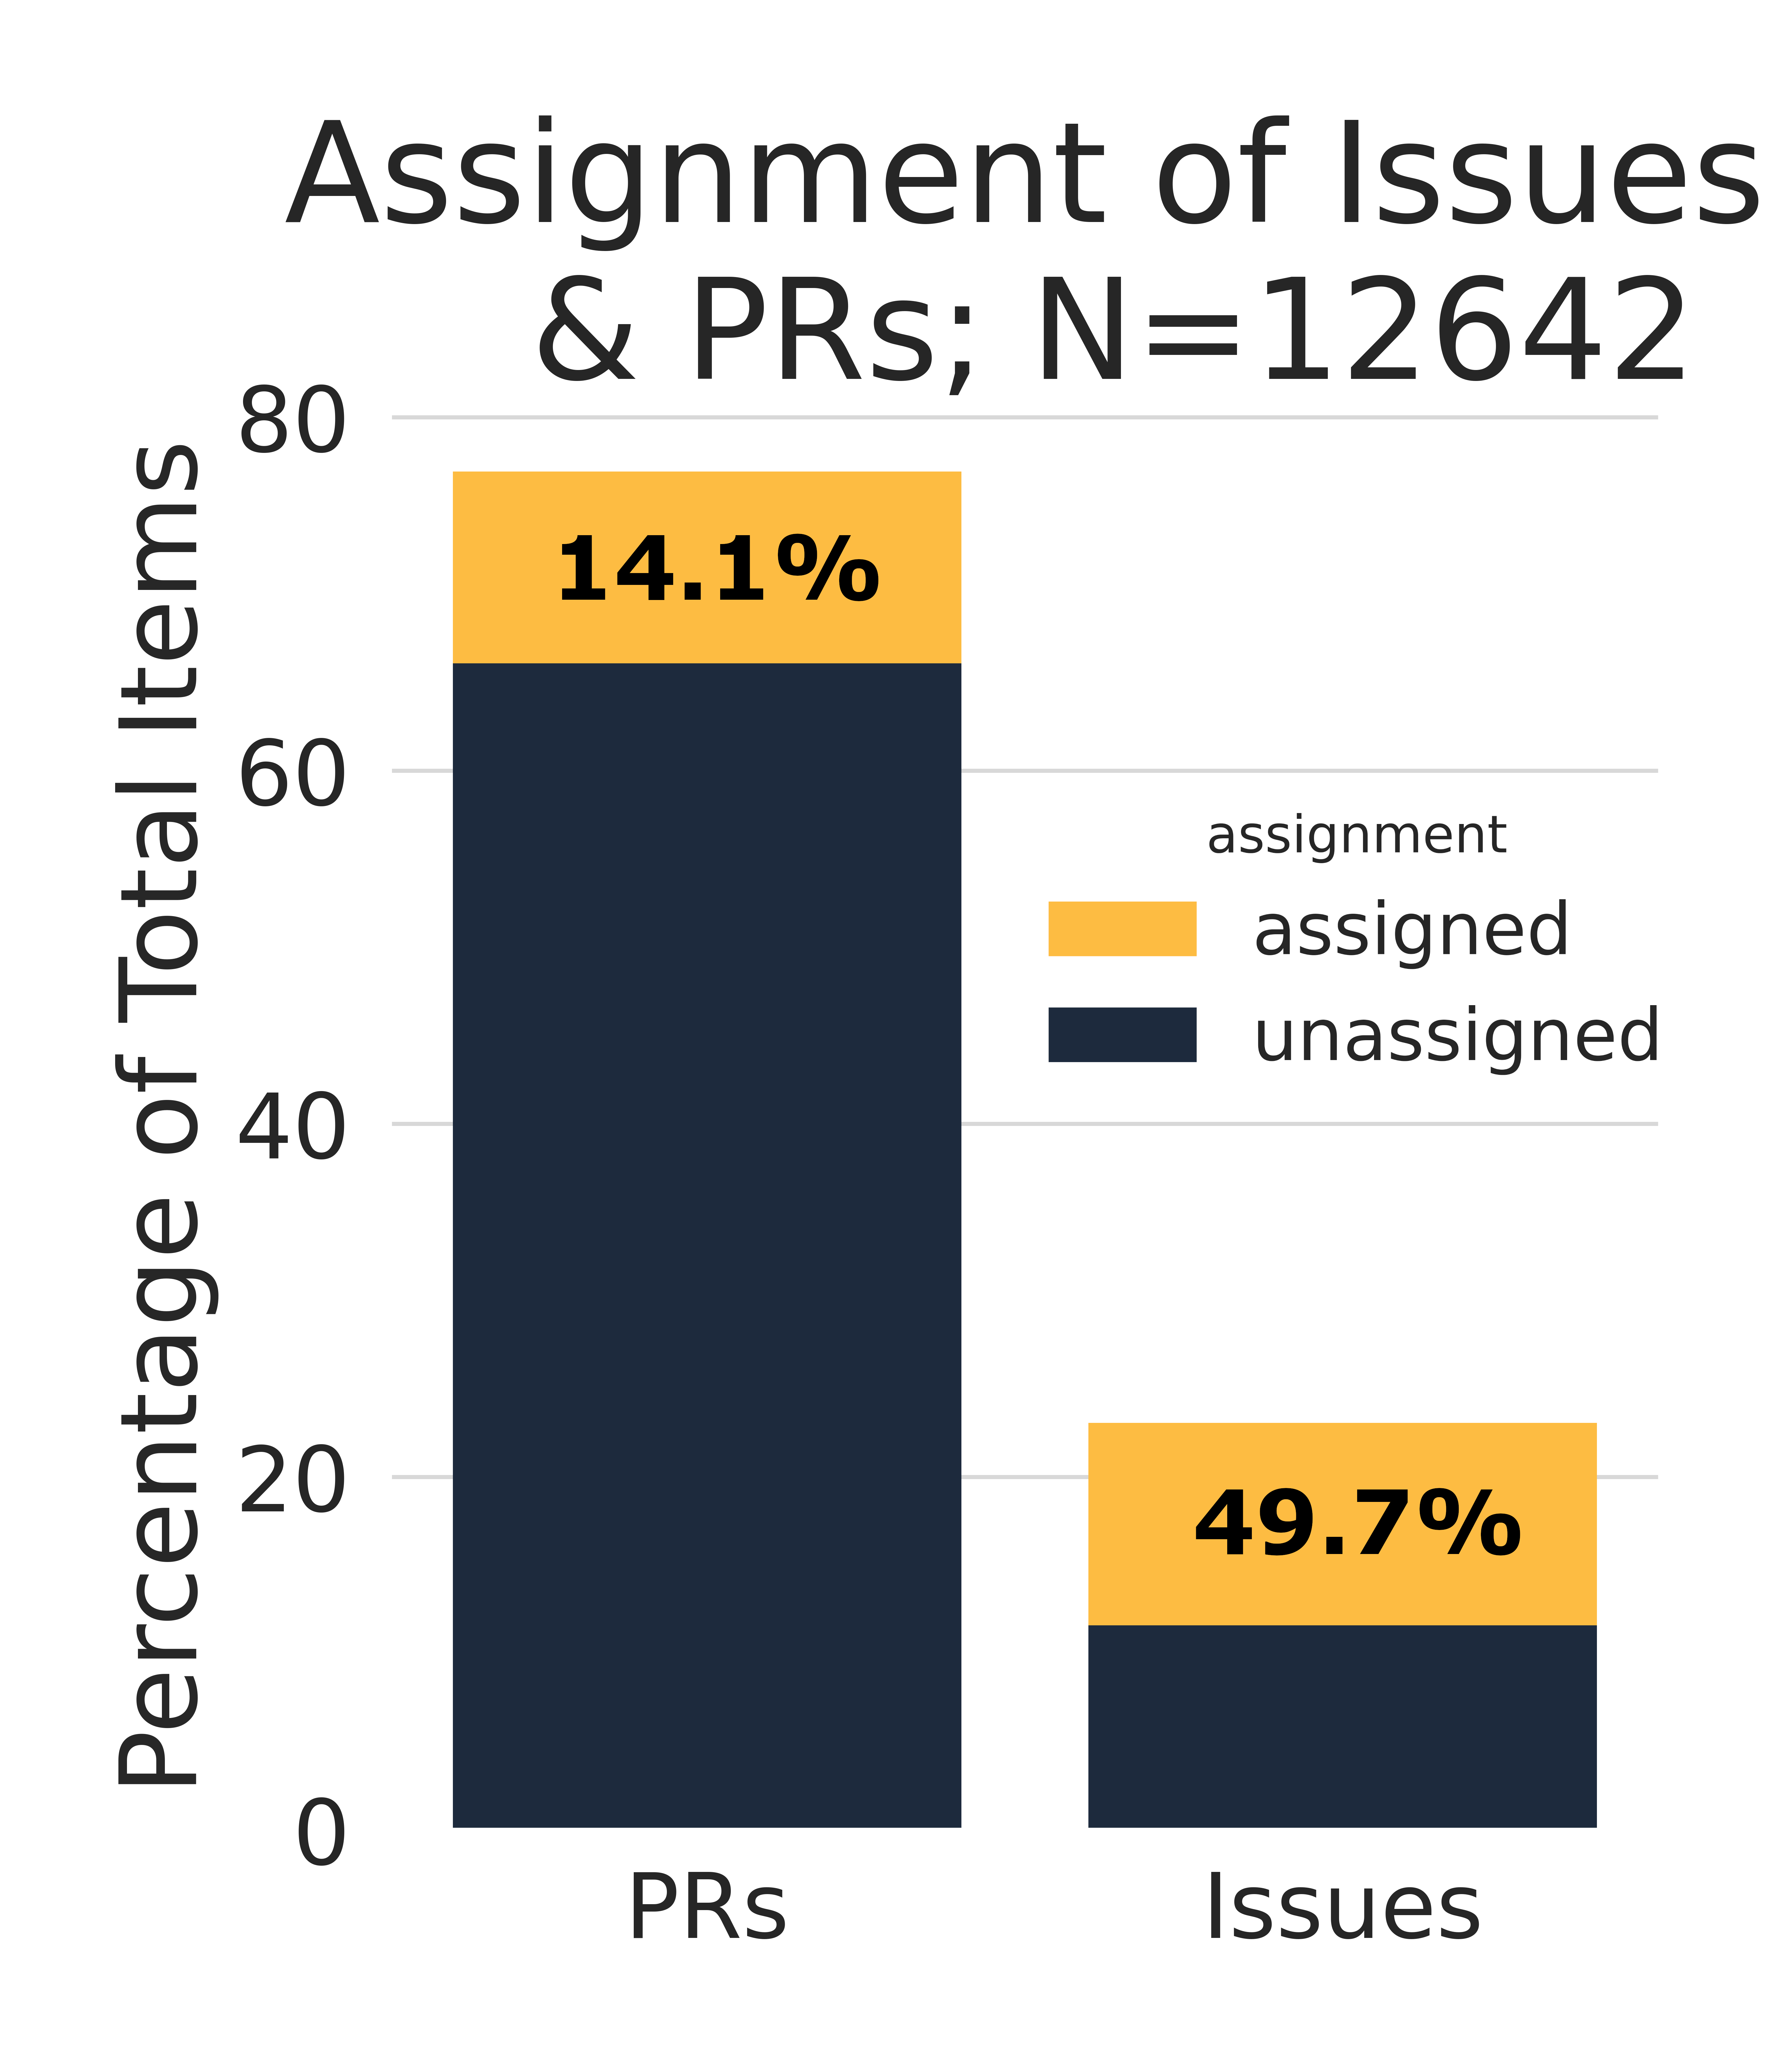
\includegraphics[width=0.60\linewidth]{Figures/bars-stacked-assignment.png}
            \includegraphics[width=0.9\linewidth]{Figures/bars-mean-commits.png}
        \end{tikzfigure}
    %\vspace*{0.4em} 
         \begin{tikzfigure}[]
        %\setlength{\belowcaptionskip}{-8pt}
            \includegraphics[width=1\linewidth]{Figures/correlations-lmplot.png}
        \end{tikzfigure}
    {\fontsize{28}{28}\selectfont 
    \begin{center}
    \begin{tabular}{ l c c} 
     %\hline
     \textbf{Category} & \textbf{N Devs} & \textbf{Devs (\%)} \\
     %\hline
     \textit{both} & 48 & \textit{18.5} \\ 
     %\hline
     issues\_only & 58 & 22.4 \\
     %\hline
     PRs\_only & 5 & 0.02 \\
     %\hline
     neither & 148 & 57.1 \\ 
     %\hline
    \end{tabular}
    \end{center}
    }    
    \vspace{0.2em}
    {\fontsize{32}{32}\selectfont 
    Commit numbers positively correlate with number of items assigned. 
    Developers assigned to 'BOTH' item types are a minority but have \textbf{$\sim$10\% higher} commit numbers than all other assignment groups. 
    \begin{tcolorbox}[colframe=white,colback=epccnavy!08, linewidth=0.8*linewidth]{        
    Are 'highly interactive' developers potential `superstars' compared to less-committed developers?
    \par}
    \end{tcolorbox}
    }
    \end{multicols}
}
\block[linewidth=5pt]{3: Using RS Developer Personas in Future Work}{
    %\vspace{1em}
    {\fontsize{38}{38}\selectfont 
    \textbf{Ask Me About Limitations...} 
    Sample potentially skews towards 'best practice'; assignment vs activity; not all commits are equal; developer metrics problems; project comparison difficulties; capturing practice changes over time; correlation vs causation.
    \vspace{0.3em} \newline
    \textbf{Future Work:}
    \begin{itemize}
        \item Using \textbf{additional properties} and \textbf{clustering analysis} to fully describe Personas
        \item Linking Personas to technical \textbf{software quality metrics} via static analysis
        \item \textbf{Distribution of Personas} within project teams
        \item \textbf{Comparing developer Personas to software effectiveness} (\textit{popularity, usage, citations})
    \end{itemize}  
    }
}
\end{columns}
\end{document}